\documentclass[1p]{elsarticle_modified}
%\bibliographystyle{elsarticle-num}

%\usepackage[colorlinks]{hyperref}
%\usepackage{abbrmath_seonhwa} %\Abb, \Ascr, \Acal ,\Abf, \Afrak
\usepackage{amsfonts}
\usepackage{amssymb}
\usepackage{amsmath}
\usepackage{amsthm}
\usepackage{scalefnt}
\usepackage{amsbsy}
\usepackage{kotex}
\usepackage{caption}
\usepackage{subfig}
\usepackage{color}
\usepackage{graphicx}
\usepackage{xcolor} %% white, black, red, green, blue, cyan, magenta, yellow
\usepackage{float}
\usepackage{setspace}
\usepackage{hyperref}

\usepackage{tikz}
\usetikzlibrary{arrows}

\usepackage{multirow}
\usepackage{array} % fixed length table
\usepackage{hhline}

%%%%%%%%%%%%%%%%%%%%%
\makeatletter
\renewcommand*\env@matrix[1][\arraystretch]{%
	\edef\arraystretch{#1}%
	\hskip -\arraycolsep
	\let\@ifnextchar\new@ifnextchar
	\array{*\c@MaxMatrixCols c}}
\makeatother %https://tex.stackexchange.com/questions/14071/how-can-i-increase-the-line-spacing-in-a-matrix
%%%%%%%%%%%%%%%

\usepackage[normalem]{ulem}

\newcommand{\msout}[1]{\ifmmode\text{\sout{\ensuremath{#1}}}\else\sout{#1}\fi}
%SOURCE: \msout is \stkout macro in https://tex.stackexchange.com/questions/20609/strikeout-in-math-mode

\newcommand{\cancel}[1]{
	\ifmmode
	{\color{red}\msout{#1}}
	\else
	{\color{red}\sout{#1}}
	\fi
}

\newcommand{\add}[1]{
	{\color{blue}\uwave{#1}}
}

\newcommand{\replace}[2]{
	\ifmmode
	{\color{red}\msout{#1}}{\color{blue}\uwave{#2}}
	\else
	{\color{red}\sout{#1}}{\color{blue}\uwave{#2}}
	\fi
}

\newcommand{\Sol}{\mathcal{S}} %segment
\newcommand{\D}{D} %diagram
\newcommand{\A}{\mathcal{A}} %arc


%%%%%%%%%%%%%%%%%%%%%%%%%%%%%5 test

\def\sl{\operatorname{\textup{SL}}(2,\Cbb)}
\def\psl{\operatorname{\textup{PSL}}(2,\Cbb)}
\def\quan{\mkern 1mu \triangleright \mkern 1mu}

\theoremstyle{definition}
\newtheorem{thm}{Theorem}[section]
\newtheorem{prop}[thm]{Proposition}
\newtheorem{lem}[thm]{Lemma}
\newtheorem{ques}[thm]{Question}
\newtheorem{cor}[thm]{Corollary}
\newtheorem{defn}[thm]{Definition}
\newtheorem{exam}[thm]{Example}
\newtheorem{rmk}[thm]{Remark}
\newtheorem{alg}[thm]{Algorithm}

\newcommand{\I}{\sqrt{-1}}
\begin{document}

%\begin{frontmatter}
%
%\title{Boundary parabolic representations of knots up to 8 crossings}
%
%%% Group authors per affiliation:
%\author{Yunhi Cho} 
%\address{Department of Mathematics, University of Seoul, Seoul, Korea}
%\ead{yhcho@uos.ac.kr}
%
%
%\author{Seonhwa Kim} %\fnref{s_kim}}
%\address{Center for Geometry and Physics, Institute for Basic Science, Pohang, 37673, Korea}
%\ead{ryeona17@ibs.re.kr}
%
%\author{Hyuk Kim}
%\address{Department of Mathematical Sciences, Seoul National University, Seoul 08826, Korea}
%\ead{hyukkim@snu.ac.kr}
%
%\author{Seokbeom Yoon}
%\address{Department of Mathematical Sciences, Seoul National University, Seoul, 08826,  Korea}
%\ead{sbyoon15@snu.ac.kr}
%
%\begin{abstract}
%We find all boundary parabolic representation of knots up to 8 crossings.
%
%\end{abstract}
%\begin{keyword}
%    \MSC[2010] 57M25 
%\end{keyword}
%
%\end{frontmatter}

%\linenumbers
%\tableofcontents
%
\newcommand\colored[1]{\textcolor{white}{\rule[-0.35ex]{0.8em}{1.4ex}}\kern-0.8em\color{red} #1}%
%\newcommand\colored[1]{\textcolor{white}{ #1}\kern-2.17ex	\textcolor{white}{ #1}\kern-1.81ex	\textcolor{white}{ #1}\kern-2.15ex\color{red}#1	}

{\Large $\underline{10_{121}~(K10a_{90})}$}

\setlength{\tabcolsep}{10pt}
\renewcommand{\arraystretch}{1.6}
\vspace{1cm}\begin{tabular}{m{100pt}>{\centering\arraybackslash}m{274pt}}
\multirow{5}{120pt}{
	\centering
	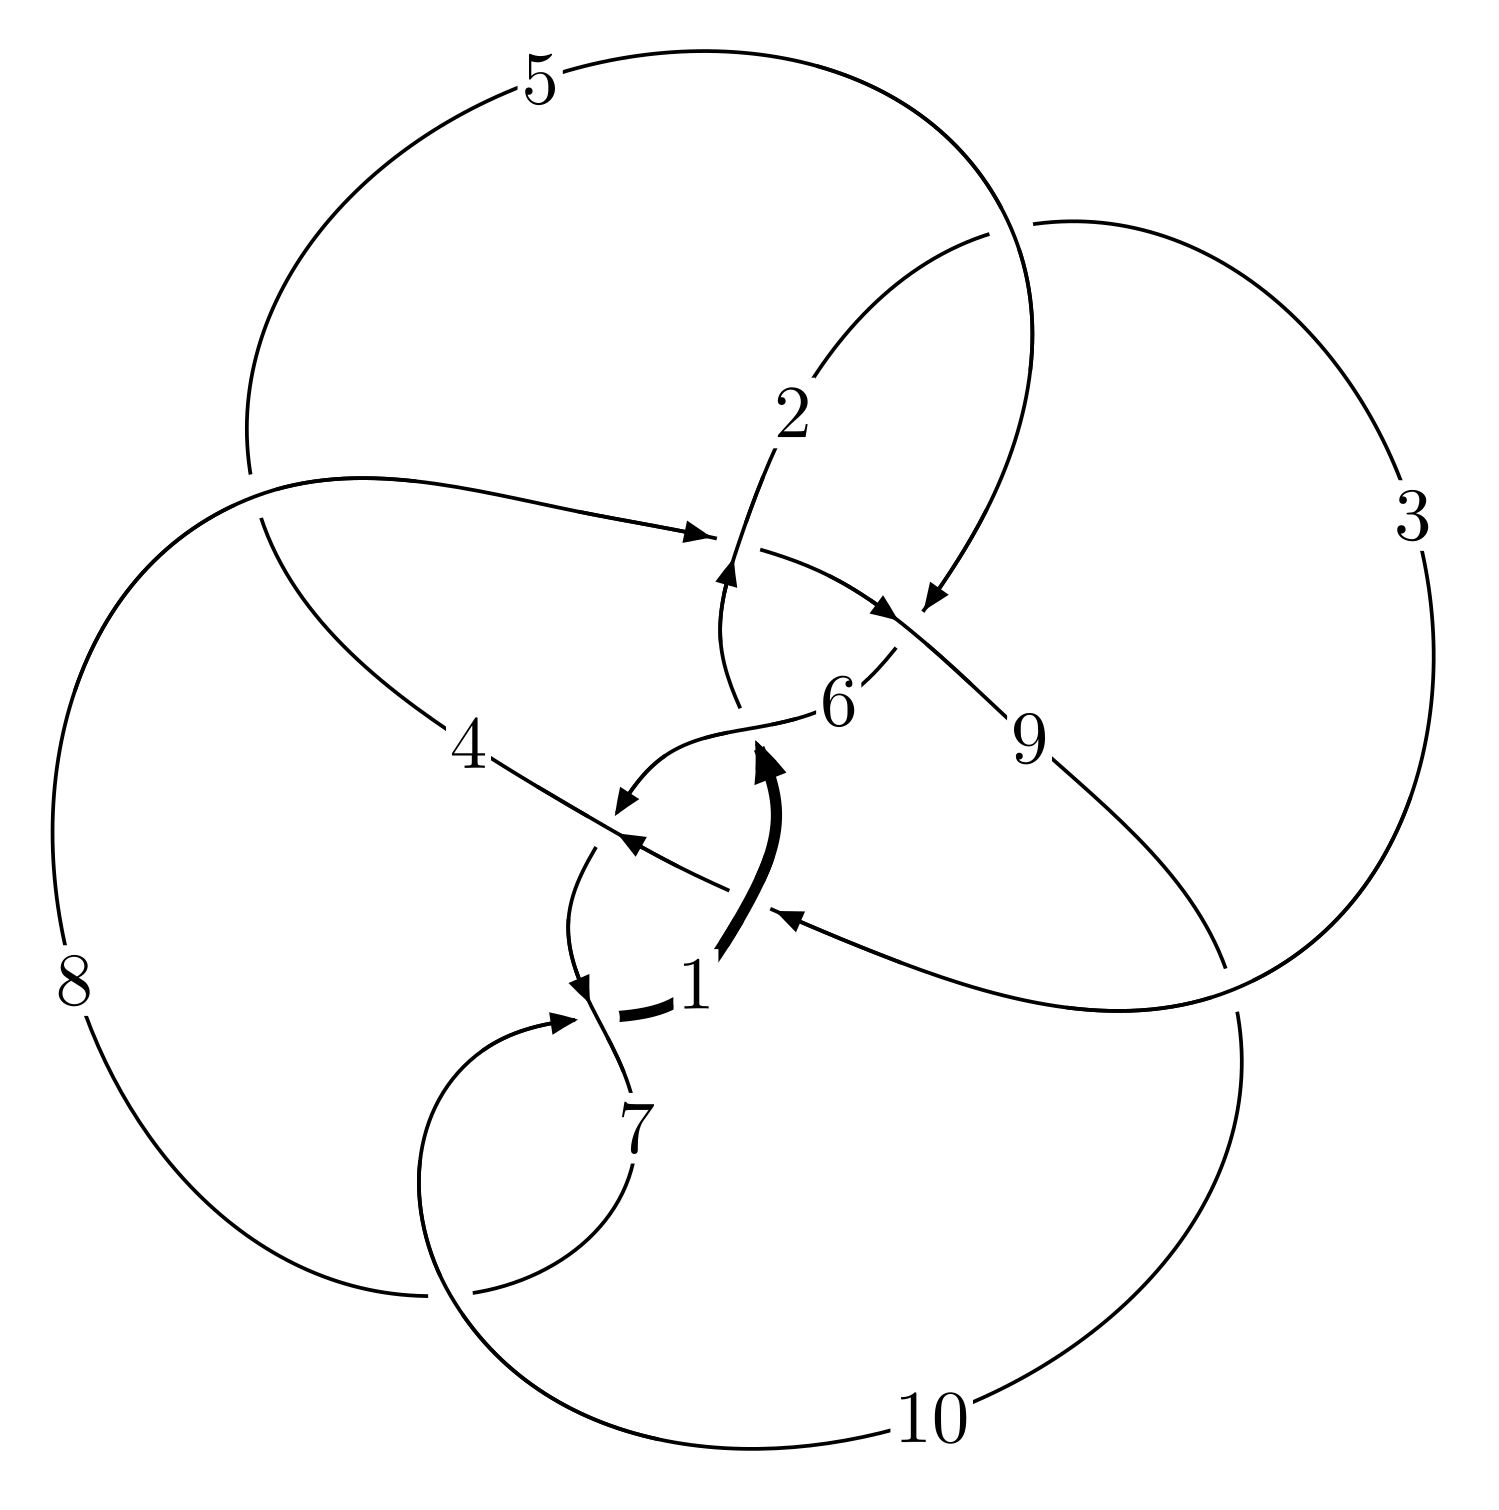
\includegraphics[width=112pt]{../../../GIT/diagram.site/Diagrams/png/205_10_121.png}\\
\ \ \ A knot diagram\footnotemark}&
\allowdisplaybreaks
\textbf{Linearized knot diagam} \\
\cline{2-2}
 &
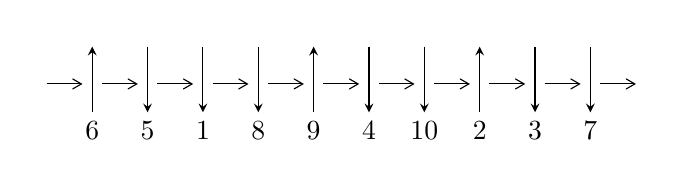
\begin{tikzpicture}[x=20pt, y=17pt]
	% nodes
	\node (C0) at (0, 0) {};
	\node (C1) at (1, 0) {};
	\node (C1U) at (1, +1) {};
	\node (C1D) at (1, -1) {6};

	\node (C2) at (2, 0) {};
	\node (C2U) at (2, +1) {};
	\node (C2D) at (2, -1) {5};

	\node (C3) at (3, 0) {};
	\node (C3U) at (3, +1) {};
	\node (C3D) at (3, -1) {1};

	\node (C4) at (4, 0) {};
	\node (C4U) at (4, +1) {};
	\node (C4D) at (4, -1) {8};

	\node (C5) at (5, 0) {};
	\node (C5U) at (5, +1) {};
	\node (C5D) at (5, -1) {9};

	\node (C6) at (6, 0) {};
	\node (C6U) at (6, +1) {};
	\node (C6D) at (6, -1) {4};

	\node (C7) at (7, 0) {};
	\node (C7U) at (7, +1) {};
	\node (C7D) at (7, -1) {10};

	\node (C8) at (8, 0) {};
	\node (C8U) at (8, +1) {};
	\node (C8D) at (8, -1) {2};

	\node (C9) at (9, 0) {};
	\node (C9U) at (9, +1) {};
	\node (C9D) at (9, -1) {3};

	\node (C10) at (10, 0) {};
	\node (C10U) at (10, +1) {};
	\node (C10D) at (10, -1) {7};
	\node (C11) at (11, 0) {};

	% arrows
	\draw[->,>={angle 60}]
	(C0) edge (C1) (C1) edge (C2) (C2) edge (C3) (C3) edge (C4) (C4) edge (C5) (C5) edge (C6) (C6) edge (C7) (C7) edge (C8) (C8) edge (C9) (C9) edge (C10) (C10) edge (C11) ;	\draw[->,>=stealth]
	(C1D) edge (C1U) (C2U) edge (C2D) (C3U) edge (C3D) (C4U) edge (C4D) (C5D) edge (C5U) (C6U) edge (C6D) (C7U) edge (C7D) (C8D) edge (C8U) (C9U) edge (C9D) (C10U) edge (C10D) ;
	\end{tikzpicture} \\
\hhline{~~} \\& 
\textbf{Solving Sequence} \\ \cline{2-2} 
 &
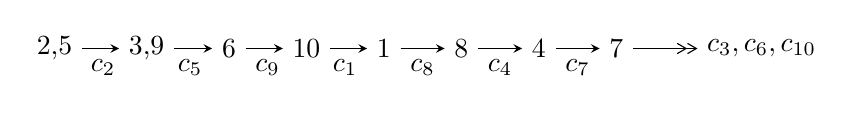
\begin{tikzpicture}[x=28pt, y=7pt]
	% node
	\node (A0) at (-1/8, 0) {2,5};
	\node (A1) at (17/16, 0) {3,9};
	\node (A2) at (17/8, 0) {6};
	\node (A3) at (25/8, 0) {10};
	\node (A4) at (33/8, 0) {1};
	\node (A5) at (41/8, 0) {8};
	\node (A6) at (49/8, 0) {4};
	\node (A7) at (57/8, 0) {7};
	\node (C1) at (1/2, -1) {$c_{2}$};
	\node (C2) at (13/8, -1) {$c_{5}$};
	\node (C3) at (21/8, -1) {$c_{9}$};
	\node (C4) at (29/8, -1) {$c_{1}$};
	\node (C5) at (37/8, -1) {$c_{8}$};
	\node (C6) at (45/8, -1) {$c_{4}$};
	\node (C7) at (53/8, -1) {$c_{7}$};
	\node (A8) at (9, 0) {$c_{3},c_{6},c_{10}$};

	% edge
	\draw[->,>=stealth]	
	(A0) edge (A1) (A1) edge (A2) (A2) edge (A3) (A3) edge (A4) (A4) edge (A5) (A5) edge (A6) (A6) edge (A7) ;
	\draw[->>,>={angle 60}]	
	(A7) edge (A8);
\end{tikzpicture} \\ 

\end{tabular} \\

\footnotetext{
The image of knot diagram is generated by the software ``\textbf{Draw programme}" developed by Andrew Bartholomew(\url{http://www.layer8.co.uk/maths/draw/index.htm\#Running-draw}), where we modified some parts for our purpose(\url{https://github.com/CATsTAILs/LinksPainter}).
}\phantom \\ \newline 
\centering \textbf{Ideals for irreducible components\footnotemark of $X_{\text{par}}$} 
 
\begin{align*}
I^u_{1}&=\langle 
-1260218947 u^{22}-19109508090 u^{21}+\cdots+984316106 b+5089661734,\\
\phantom{I^u_{1}}&\phantom{= \langle  }-2544830867 u^{22}-38196855978 u^{21}+\cdots+1968632212 a+17497959996,\\
\phantom{I^u_{1}}&\phantom{= \langle  }u^{23}+16 u^{22}+\cdots-10 u-4\rangle \\
I^u_{2}&=\langle 
111 u^{10} a^3+343 u^{10} a^2+\cdots-317 a-203,\;- u^{10} a^3+5 u^{10} a^2+\cdots+9 a^2+12,\\
\phantom{I^u_{2}}&\phantom{= \langle  }u^{11}-5 u^{10}+12 u^9-15 u^8+8 u^7+4 u^6-8 u^5+3 u^4+3 u^3-3 u^2+1\rangle \\
I^u_{3}&=\langle 
u^9-5 u^8+11 u^7-12 u^6+5 u^5+3 u^4-5 u^3+3 u^2+b+u-2,\\
\phantom{I^u_{3}}&\phantom{= \langle  }2 u^9-9 u^8+19 u^7-21 u^6+12 u^5- u^4-3 u^3+3 u^2+a+u-1,\\
\phantom{I^u_{3}}&\phantom{= \langle  }u^{10}-5 u^9+12 u^8-16 u^7+12 u^6-3 u^5-3 u^4+4 u^3- u^2- u+1\rangle \\
\\
\end{align*}
\raggedright * 3 irreducible components of $\dim_{\mathbb{C}}=0$, with total 77 representations.\\
\footnotetext{All coefficients of polynomials are rational numbers. But the coefficients are sometimes approximated in decimal forms when there is not enough margin.}
\newpage
\renewcommand{\arraystretch}{1}
\centering \section*{I. $I^u_{1}= \langle -1.26\times10^{9} u^{22}-1.91\times10^{10} u^{21}+\cdots+9.84\times10^{8} b+5.09\times10^{9},\;-2.54\times10^{9} u^{22}-3.82\times10^{10} u^{21}+\cdots+1.97\times10^{9} a+1.75\times10^{10},\;u^{23}+16 u^{22}+\cdots-10 u-4 \rangle$}
\flushleft \textbf{(i) Arc colorings}\\
\begin{tabular}{m{7pt} m{180pt} m{7pt} m{180pt} }
\flushright $a_{2}=$&$\begin{pmatrix}1\\0\end{pmatrix}$ \\
\flushright $a_{5}=$&$\begin{pmatrix}0\\u\end{pmatrix}$ \\
\flushright $a_{3}=$&$\begin{pmatrix}1\\u^2\end{pmatrix}$ \\
\flushright $a_{9}=$&$\begin{pmatrix}1.29269 u^{22}+19.4027 u^{21}+\cdots-9.50831 u-8.88838\\1.28030 u^{22}+19.4140 u^{21}+\cdots-4.03851 u-5.17076\end{pmatrix}$ \\
\flushright $a_{6}=$&$\begin{pmatrix}0.319249 u^{22}+5.03061 u^{21}+\cdots+6.76619 u-4.03209\\0.0773747 u^{22}+0.861665 u^{21}+\cdots+1.83960 u-1.27700\end{pmatrix}$ \\
\flushright $a_{10}=$&$\begin{pmatrix}1.08318 u^{22}+16.7864 u^{21}+\cdots-13.1020 u-8.83882\\-0.0242790 u^{22}-0.125186 u^{21}+\cdots+2.48170 u-2.22746\end{pmatrix}$ \\
\flushright $a_{1}=$&$\begin{pmatrix}1.02071 u^{22}+13.6913 u^{21}+\cdots-4.25396 u+6.74097\\2.26372 u^{22}+33.8581 u^{21}+\cdots-16.4513 u-3.77333\end{pmatrix}$ \\
\flushright $a_{8}=$&$\begin{pmatrix}0.0123908 u^{22}-0.0112566 u^{21}+\cdots-5.46979 u-3.71763\\1.28030 u^{22}+19.4140 u^{21}+\cdots-4.03851 u-5.17076\end{pmatrix}$ \\
\flushright $a_{4}=$&$\begin{pmatrix}0.540830 u^{22}+8.50923 u^{21}+\cdots+5.59024 u-1.78760\\-0.298956 u^{22}-4.34029 u^{21}+\cdots+1.33635 u-0.967496\end{pmatrix}$ \\
\flushright $a_{7}=$&$\begin{pmatrix}-0.221415 u^{22}-3.51881 u^{21}+\cdots-1.62252 u-3.99396\\0.519049 u^{22}+7.71688 u^{21}+\cdots+1.74955 u-3.39079\end{pmatrix}$\\&\end{tabular}
\flushleft \textbf{(ii) Obstruction class $= -1$}\\~\\
\flushleft \textbf{(iii) Cusp Shapes $= -\frac{3396085143}{492158053} u^{22}-\frac{53190862554}{492158053} u^{21}+\cdots+\frac{29461471174}{492158053} u+\frac{13339530290}{492158053}$}\\~\\
\newpage\renewcommand{\arraystretch}{1}
\flushleft \textbf{(iv) u-Polynomials at the component}\newline \\
\begin{tabular}{m{50pt}|m{274pt}}
Crossings & \hspace{64pt}u-Polynomials at each crossing \\
\hline $$\begin{aligned}c_{1}\end{aligned}$$&$\begin{aligned}
&u^{23}-19 u^{22}+\cdots-18432 u+2048
\end{aligned}$\\
\hline $$\begin{aligned}c_{2}\end{aligned}$$&$\begin{aligned}
&u^{23}-16 u^{22}+\cdots-10 u+4
\end{aligned}$\\
\hline $$\begin{aligned}c_{3},c_{6}\end{aligned}$$&$\begin{aligned}
&u^{23}+u^{22}+\cdots+2 u+1
\end{aligned}$\\
\hline $$\begin{aligned}c_{4},c_{9}\end{aligned}$$&$\begin{aligned}
&u^{23}+u^{22}+\cdots+u+1
\end{aligned}$\\
\hline $$\begin{aligned}c_{5},c_{8}\end{aligned}$$&$\begin{aligned}
&u^{23}- u^{22}+\cdots+2 u+1
\end{aligned}$\\
\hline $$\begin{aligned}c_{7},c_{10}\end{aligned}$$&$\begin{aligned}
&u^{23}-10 u^{22}+\cdots-108 u+16
\end{aligned}$\\
\hline
\end{tabular}\\~\\
\newpage\renewcommand{\arraystretch}{1}
\flushleft \textbf{(v) Riley Polynomials at the component}\newline \\
\begin{tabular}{m{50pt}|m{274pt}}
Crossings & \hspace{64pt}Riley Polynomials at each crossing \\
\hline $$\begin{aligned}c_{1}\end{aligned}$$&$\begin{aligned}
&y^{23}+9 y^{22}+\cdots+2097152 y-4194304
\end{aligned}$\\
\hline $$\begin{aligned}c_{2}\end{aligned}$$&$\begin{aligned}
&y^{23}-2 y^{22}+\cdots+252 y-16
\end{aligned}$\\
\hline $$\begin{aligned}c_{3},c_{6}\end{aligned}$$&$\begin{aligned}
&y^{23}+9 y^{22}+\cdots-16 y-1
\end{aligned}$\\
\hline $$\begin{aligned}c_{4},c_{9}\end{aligned}$$&$\begin{aligned}
&y^{23}-7 y^{22}+\cdots- y-1
\end{aligned}$\\
\hline $$\begin{aligned}c_{5},c_{8}\end{aligned}$$&$\begin{aligned}
&y^{23}-3 y^{22}+\cdots+6 y-1
\end{aligned}$\\
\hline $$\begin{aligned}c_{7},c_{10}\end{aligned}$$&$\begin{aligned}
&y^{23}+16 y^{22}+\cdots-1360 y-256
\end{aligned}$\\
\hline
\end{tabular}\\~\\
\newpage\flushleft \textbf{(vi) Complex Volumes and Cusp Shapes}
$$\begin{array}{c|c|c}  
\text{Solutions to }I^u_{1}& \I (\text{vol} + \sqrt{-1}CS) & \text{Cusp shape}\\
 \hline 
\begin{aligned}
u &= -0.799030 + 0.571303 I \\
a &= -0.12013 - 1.57743 I \\
b &= -0.99718 - 1.19178 I\end{aligned}
 & \phantom{-}1.35281 + 4.50771 I & \phantom{-}12.5679 - 8.0453 I \\ \hline\begin{aligned}
u &= -0.799030 - 0.571303 I \\
a &= -0.12013 + 1.57743 I \\
b &= -0.99718 + 1.19178 I\end{aligned}
 & \phantom{-}1.35281 - 4.50771 I & \phantom{-}12.5679 + 8.0453 I \\ \hline\begin{aligned}
u &= \phantom{-}0.924432\phantom{ +0.000000I} \\
a &= -0.417135\phantom{ +0.000000I} \\
b &= \phantom{-}0.385613\phantom{ +0.000000I}\end{aligned}
 & -1.38648\phantom{ +0.000000I} & -7.37670\phantom{ +0.000000I} \\ \hline\begin{aligned}
u &= -0.517217 + 1.045830 I \\
a &= -0.047708 + 0.890847 I \\
b &= \phantom{-}0.906994 + 0.510655 I\end{aligned}
 & \phantom{-}6.24675 - 0.93599 I & \phantom{-}3.26085 + 0.04991 I \\ \hline\begin{aligned}
u &= -0.517217 - 1.045830 I \\
a &= -0.047708 - 0.890847 I \\
b &= \phantom{-}0.906994 - 0.510655 I\end{aligned}
 & \phantom{-}6.24675 + 0.93599 I & \phantom{-}3.26085 - 0.04991 I \\ \hline\begin{aligned}
u &= -1.119710 + 0.513718 I \\
a &= -0.452909 - 0.773390 I \\
b &= -0.904431 - 0.633306 I\end{aligned}
 & \phantom{-}0.95729 + 2.04351 I & \phantom{-}2.51837 - 2.36281 I \\ \hline\begin{aligned}
u &= -1.119710 - 0.513718 I \\
a &= -0.452909 + 0.773390 I \\
b &= -0.904431 + 0.633306 I\end{aligned}
 & \phantom{-}0.95729 - 2.04351 I & \phantom{-}2.51837 + 2.36281 I \\ \hline\begin{aligned}
u &= -0.587912 + 0.172198 I \\
a &= -0.88228 - 1.27862 I \\
b &= -0.738880 - 0.599789 I\end{aligned}
 & \phantom{-}1.10859 + 1.69807 I & \phantom{-}0.99491 - 2.62569 I \\ \hline\begin{aligned}
u &= -0.587912 - 0.172198 I \\
a &= -0.88228 + 1.27862 I \\
b &= -0.738880 + 0.599789 I\end{aligned}
 & \phantom{-}1.10859 - 1.69807 I & \phantom{-}0.99491 + 2.62569 I \\ \hline\begin{aligned}
u &= \phantom{-}0.267486 + 0.510215 I \\
a &= \phantom{-}0.57156 - 1.32428 I \\
b &= -0.828550 + 0.062607 I\end{aligned}
 & \phantom{-}2.14619 - 2.15516 I & \phantom{-}1.26567 + 4.32711 I\\
 \hline 
 \end{array}$$\newpage$$\begin{array}{c|c|c}  
\text{Solutions to }I^u_{1}& \I (\text{vol} + \sqrt{-1}CS) & \text{Cusp shape}\\
 \hline 
\begin{aligned}
u &= \phantom{-}0.267486 - 0.510215 I \\
a &= \phantom{-}0.57156 + 1.32428 I \\
b &= -0.828550 - 0.062607 I\end{aligned}
 & \phantom{-}2.14619 + 2.15516 I & \phantom{-}1.26567 - 4.32711 I \\ \hline\begin{aligned}
u &= -1.14560 + 0.90839 I \\
a &= \phantom{-}0.060381 + 1.065800 I \\
b &= \phantom{-}1.03734 + 1.16613 I\end{aligned}
 & -4.47926 + 10.82160 I & -7.18200 - 7.95225 I \\ \hline\begin{aligned}
u &= -1.14560 - 0.90839 I \\
a &= \phantom{-}0.060381 - 1.065800 I \\
b &= \phantom{-}1.03734 - 1.16613 I\end{aligned}
 & -4.47926 - 10.82160 I & -7.18200 + 7.95225 I \\ \hline\begin{aligned}
u &= -1.14496 + 1.09496 I \\
a &= \phantom{-}0.038158 - 1.004390 I \\
b &= -1.05609 - 1.19178 I\end{aligned}
 & -0.6004 + 16.9749 I & \phantom{-0.000000 } 0. - 9.34400 I \\ \hline\begin{aligned}
u &= -1.14496 - 1.09496 I \\
a &= \phantom{-}0.038158 + 1.004390 I \\
b &= -1.05609 + 1.19178 I\end{aligned}
 & -0.6004 - 16.9749 I & \phantom{-0.000000 -}0. + 9.34400 I \\ \hline\begin{aligned}
u &= \phantom{-}0.257593 + 0.139438 I \\
a &= -3.87302 + 0.15811 I \\
b &= \phantom{-}1.019710 + 0.499316 I\end{aligned}
 & \phantom{-}1.57996 + 1.95049 I & \phantom{-}0.00371 - 3.34610 I \\ \hline\begin{aligned}
u &= \phantom{-}0.257593 - 0.139438 I \\
a &= -3.87302 - 0.15811 I \\
b &= \phantom{-}1.019710 - 0.499316 I\end{aligned}
 & \phantom{-}1.57996 - 1.95049 I & \phantom{-}0.00371 + 3.34610 I \\ \hline\begin{aligned}
u &= -1.37621 + 1.06752 I \\
a &= \phantom{-}0.189943 + 0.547859 I \\
b &= \phantom{-}0.846254 + 0.551200 I\end{aligned}
 & \phantom{-}3.21418 + 8.47524 I & \phantom{-0.000000 } 0 \\ \hline\begin{aligned}
u &= -1.37621 - 1.06752 I \\
a &= \phantom{-}0.189943 - 0.547859 I \\
b &= \phantom{-}0.846254 - 0.551200 I\end{aligned}
 & \phantom{-}3.21418 - 8.47524 I & \phantom{-0.000000 } 0 \\ \hline\begin{aligned}
u &= -0.84300 + 1.61883 I \\
a &= \phantom{-}0.299587 - 0.003010 I \\
b &= \phantom{-}0.247680 - 0.487517 I\end{aligned}
 & -2.90076 - 2.91786 I & \phantom{-0.000000 } 0\\
 \hline 
 \end{array}$$\newpage$$\begin{array}{c|c|c}  
\text{Solutions to }I^u_{1}& \I (\text{vol} + \sqrt{-1}CS) & \text{Cusp shape}\\
 \hline 
\begin{aligned}
u &= -0.84300 - 1.61883 I \\
a &= \phantom{-}0.299587 + 0.003010 I \\
b &= \phantom{-}0.247680 + 0.487517 I\end{aligned}
 & -2.90076 + 2.91786 I & \phantom{-0.000000 } 0 \\ \hline\begin{aligned}
u &= -1.45365 + 1.27820 I \\
a &= -0.325009 + 0.193081 I \\
b &= -0.225654 + 0.696100 I\end{aligned}
 & -0.52992 - 8.08521 I & \phantom{-0.000000 } 0 \\ \hline\begin{aligned}
u &= -1.45365 - 1.27820 I \\
a &= -0.325009 - 0.193081 I \\
b &= -0.225654 - 0.696100 I\end{aligned}
 & -0.52992 + 8.08521 I & \phantom{-0.000000 } 0\\
 \hline 
 \end{array}$$\newpage\newpage\renewcommand{\arraystretch}{1}
\centering \section*{II. $I^u_{2}= \langle 111 u^{10} a^3+343 u^{10} a^2+\cdots-317 a-203,\;- u^{10} a^3+5 u^{10} a^2+\cdots+9 a^2+12,\;u^{11}-5 u^{10}+\cdots-3 u^2+1 \rangle$}
\flushleft \textbf{(i) Arc colorings}\\
\begin{tabular}{m{7pt} m{180pt} m{7pt} m{180pt} }
\flushright $a_{2}=$&$\begin{pmatrix}1\\0\end{pmatrix}$ \\
\flushright $a_{5}=$&$\begin{pmatrix}0\\u\end{pmatrix}$ \\
\flushright $a_{3}=$&$\begin{pmatrix}1\\u^2\end{pmatrix}$ \\
\flushright $a_{9}=$&$\begin{pmatrix}a\\-0.350158 a^{3} u^{10}-1.08202 a^{2} u^{10}+\cdots+a+0.640379\end{pmatrix}$ \\
\flushright $a_{6}=$&$\begin{pmatrix}a^2 u\\-0.0820189 a^{3} u^{10}+0.350158 a^{2} u^{10}+\cdots-a+0.996845\end{pmatrix}$ \\
\flushright $a_{10}=$&$\begin{pmatrix}0.350158 a^{3} u^{10}+1.08202 a^{2} u^{10}+\cdots-1.04101 a^{2}-0.640379\\0.0504732 a^{3} u^{10}-0.753943 a^{2} u^{10}+\cdots+0.876972 a^{2}+0.0788644\end{pmatrix}$ \\
\flushright $a_{1}=$&$\begin{pmatrix}0.0410095 a^{3} u^{10}-0.675079 a^{2} u^{10}+\cdots+a+0.501577\\-0.0820189 a^{3} u^{10}+0.350158 a^{2} u^{10}+\cdots-a-0.00315457\end{pmatrix}$ \\
\flushright $a_{8}=$&$\begin{pmatrix}0.350158 a^{3} u^{10}+1.08202 a^{2} u^{10}+\cdots-1.04101 a^{2}-0.640379\\-0.350158 a^{3} u^{10}-1.08202 a^{2} u^{10}+\cdots+a+0.640379\end{pmatrix}$ \\
\flushright $a_{4}=$&$\begin{pmatrix}-0.328076 a^{3} u^{10}+0.400631 a^{2} u^{10}+\cdots-a-0.0126183\\0.410095 a^{3} u^{10}-0.750789 a^{2} u^{10}+\cdots+2 a-0.984227\end{pmatrix}$ \\
\flushright $a_{7}=$&$\begin{pmatrix}-0.451104 a^{3} u^{10}+0.425868 a^{2} u^{10}+\cdots-0.712934 a^{2}+0.482650\\0.246057 a^{3} u^{10}-1.05047 a^{2} u^{10}+\cdots+2 a+0.00946372\end{pmatrix}$\\&\end{tabular}
\flushleft \textbf{(ii) Obstruction class $= -1$}\\~\\
\flushleft \textbf{(iii) Cusp Shapes $= \frac{104}{317} u^{10} a^3-\frac{444}{317} u^{10} a^2+\cdots+4 a-\frac{6970}{317}$}\\~\\
\newpage\renewcommand{\arraystretch}{1}
\flushleft \textbf{(iv) u-Polynomials at the component}\newline \\
\begin{tabular}{m{50pt}|m{274pt}}
Crossings & \hspace{64pt}u-Polynomials at each crossing \\
\hline $$\begin{aligned}c_{1}\end{aligned}$$&$\begin{aligned}
&(u^2+u+1)^{22}
\end{aligned}$\\
\hline $$\begin{aligned}c_{2}\end{aligned}$$&$\begin{aligned}
&(u^{11}+5 u^{10}+12 u^9+15 u^8+8 u^7-4 u^6-8 u^5-3 u^4+3 u^3+3 u^2-1)^4
\end{aligned}$\\
\hline $$\begin{aligned}c_{3},c_{6}\end{aligned}$$&$\begin{aligned}
&u^{44}+u^{43}+\cdots-8 u+1
\end{aligned}$\\
\hline $$\begin{aligned}c_{4},c_{9}\end{aligned}$$&$\begin{aligned}
&u^{44}- u^{43}+\cdots-918 u+289
\end{aligned}$\\
\hline $$\begin{aligned}c_{5},c_{8}\end{aligned}$$&$\begin{aligned}
&u^{44}-3 u^{43}+\cdots+14 u+1
\end{aligned}$\\
\hline $$\begin{aligned}c_{7},c_{10}\end{aligned}$$&$\begin{aligned}
&(u^{11}+3 u^{10}+\cdots+2 u+1)^{4}
\end{aligned}$\\
\hline
\end{tabular}\\~\\
\newpage\renewcommand{\arraystretch}{1}
\flushleft \textbf{(v) Riley Polynomials at the component}\newline \\
\begin{tabular}{m{50pt}|m{274pt}}
Crossings & \hspace{64pt}Riley Polynomials at each crossing \\
\hline $$\begin{aligned}c_{1}\end{aligned}$$&$\begin{aligned}
&(y^2+y+1)^{22}
\end{aligned}$\\
\hline $$\begin{aligned}c_{2}\end{aligned}$$&$\begin{aligned}
&(y^{11}- y^{10}+\cdots+6 y-1)^{4}
\end{aligned}$\\
\hline $$\begin{aligned}c_{3},c_{6}\end{aligned}$$&$\begin{aligned}
&y^{44}-9 y^{43}+\cdots-8 y+1
\end{aligned}$\\
\hline $$\begin{aligned}c_{4},c_{9}\end{aligned}$$&$\begin{aligned}
&y^{44}-13 y^{43}+\cdots-899368 y+83521
\end{aligned}$\\
\hline $$\begin{aligned}c_{5},c_{8}\end{aligned}$$&$\begin{aligned}
&y^{44}+15 y^{43}+\cdots-56 y+1
\end{aligned}$\\
\hline $$\begin{aligned}c_{7},c_{10}\end{aligned}$$&$\begin{aligned}
&(y^{11}+7 y^{10}+\cdots-6 y-1)^{4}
\end{aligned}$\\
\hline
\end{tabular}\\~\\
\newpage\flushleft \textbf{(vi) Complex Volumes and Cusp Shapes}
$$\begin{array}{c|c|c}  
\text{Solutions to }I^u_{2}& \I (\text{vol} + \sqrt{-1}CS) & \text{Cusp shape}\\
 \hline 
\begin{aligned}
u &= \phantom{-}0.326966 + 0.916688 I \\
a &= -0.038498 - 1.048450 I \\
b &= \phantom{-}0.80389 - 1.55903 I\end{aligned}
 & \phantom{-}2.98579 - 7.03062 I & \phantom{-}1.84059 + 9.69161 I \\ \hline\begin{aligned}
u &= \phantom{-}0.326966 + 0.916688 I \\
a &= -0.281007 - 1.284950 I \\
b &= \phantom{-}0.1356230 + 0.0379857 I\end{aligned}
 & \phantom{-}2.98579 - 2.97085 I & \phantom{-}1.84059 + 2.76341 I \\ \hline\begin{aligned}
u &= \phantom{-}0.326966 + 0.916688 I \\
a &= \phantom{-}1.23128 + 1.31612 I \\
b &= -0.948517 + 0.378099 I\end{aligned}
 & \phantom{-}2.98579 - 7.03062 I & \phantom{-}1.84059 + 9.69161 I \\ \hline\begin{aligned}
u &= \phantom{-}0.326966 + 0.916688 I \\
a &= -0.083576 + 0.118139 I \\
b &= -1.086020 + 0.677732 I\end{aligned}
 & \phantom{-}2.98579 - 2.97085 I & \phantom{-}1.84059 + 2.76341 I \\ \hline\begin{aligned}
u &= \phantom{-}0.326966 - 0.916688 I \\
a &= -0.038498 + 1.048450 I \\
b &= \phantom{-}0.80389 + 1.55903 I\end{aligned}
 & \phantom{-}2.98579 + 7.03062 I & \phantom{-}1.84059 - 9.69161 I \\ \hline\begin{aligned}
u &= \phantom{-}0.326966 - 0.916688 I \\
a &= -0.281007 + 1.284950 I \\
b &= \phantom{-}0.1356230 - 0.0379857 I\end{aligned}
 & \phantom{-}2.98579 + 2.97085 I & \phantom{-}1.84059 - 2.76341 I \\ \hline\begin{aligned}
u &= \phantom{-}0.326966 - 0.916688 I \\
a &= \phantom{-}1.23128 - 1.31612 I \\
b &= -0.948517 - 0.378099 I\end{aligned}
 & \phantom{-}2.98579 + 7.03062 I & \phantom{-}1.84059 - 9.69161 I \\ \hline\begin{aligned}
u &= \phantom{-}0.326966 - 0.916688 I \\
a &= -0.083576 - 0.118139 I \\
b &= -1.086020 - 0.677732 I\end{aligned}
 & \phantom{-}2.98579 + 2.97085 I & \phantom{-}1.84059 - 2.76341 I \\ \hline\begin{aligned}
u &= \phantom{-}0.864248 + 0.407709 I \\
a &= -0.129704 + 0.797794 I \\
b &= -1.09220 + 1.32253 I\end{aligned}
 & -2.06894 - 4.27767 I & -9.63582 + 8.52770 I \\ \hline\begin{aligned}
u &= \phantom{-}0.864248 + 0.407709 I \\
a &= -1.193510 - 0.275075 I \\
b &= \phantom{-}0.002110 - 0.500193 I\end{aligned}
 & -2.06894 - 0.21790 I & -9.63582 + 1.59949 I\\
 \hline 
 \end{array}$$\newpage$$\begin{array}{c|c|c}  
\text{Solutions to }I^u_{2}& \I (\text{vol} + \sqrt{-1}CS) & \text{Cusp shape}\\
 \hline 
\begin{aligned}
u &= \phantom{-}0.864248 + 0.407709 I \\
a &= \phantom{-}0.221332 + 0.474348 I \\
b &= \phantom{-}0.919334 + 0.724336 I\end{aligned}
 & -2.06894 - 0.21790 I & -9.63582 + 1.59949 I \\ \hline\begin{aligned}
u &= \phantom{-}0.864248 + 0.407709 I \\
a &= \phantom{-}0.44322 - 1.73936 I \\
b &= \phantom{-}0.437365 - 0.636610 I\end{aligned}
 & -2.06894 - 4.27767 I & -9.63582 + 8.52770 I \\ \hline\begin{aligned}
u &= \phantom{-}0.864248 - 0.407709 I \\
a &= -0.129704 - 0.797794 I \\
b &= -1.09220 - 1.32253 I\end{aligned}
 & -2.06894 + 4.27767 I & -9.63582 - 8.52770 I \\ \hline\begin{aligned}
u &= \phantom{-}0.864248 - 0.407709 I \\
a &= -1.193510 + 0.275075 I \\
b &= \phantom{-}0.002110 + 0.500193 I\end{aligned}
 & -2.06894 + 0.21790 I & -9.63582 - 1.59949 I \\ \hline\begin{aligned}
u &= \phantom{-}0.864248 - 0.407709 I \\
a &= \phantom{-}0.221332 - 0.474348 I \\
b &= \phantom{-}0.919334 - 0.724336 I\end{aligned}
 & -2.06894 + 0.21790 I & -9.63582 - 1.59949 I \\ \hline\begin{aligned}
u &= \phantom{-}0.864248 - 0.407709 I \\
a &= \phantom{-}0.44322 + 1.73936 I \\
b &= \phantom{-}0.437365 + 0.636610 I\end{aligned}
 & -2.06894 + 4.27767 I & -9.63582 - 8.52770 I \\ \hline\begin{aligned}
u &= -0.577598 + 0.283449 I \\
a &= -0.081013 + 0.913235 I \\
b &= -1.57832 + 1.34962 I\end{aligned}
 & \phantom{-}0.11530 + 7.95431 I & -9.1705 - 13.4876 I \\ \hline\begin{aligned}
u &= -0.577598 + 0.283449 I \\
a &= \phantom{-}0.76538 - 1.71451 I \\
b &= -0.918479 - 0.926010 I\end{aligned}
 & \phantom{-}0.11530 + 3.89454 I & -9.17045 - 6.55945 I \\ \hline\begin{aligned}
u &= -0.577598 + 0.283449 I \\
a &= -0.64749 - 1.92095 I \\
b &= -0.043897 - 1.207240 I\end{aligned}
 & \phantom{-}0.11530 + 3.89454 I & -9.17045 - 6.55945 I \\ \hline\begin{aligned}
u &= -0.577598 + 0.283449 I \\
a &= -3.12633 + 0.80240 I \\
b &= \phantom{-}0.212063 + 0.550445 I\end{aligned}
 & \phantom{-}0.11530 + 7.95431 I & -9.1705 - 13.4876 I\\
 \hline 
 \end{array}$$\newpage$$\begin{array}{c|c|c}  
\text{Solutions to }I^u_{2}& \I (\text{vol} + \sqrt{-1}CS) & \text{Cusp shape}\\
 \hline 
\begin{aligned}
u &= -0.577598 - 0.283449 I \\
a &= -0.081013 - 0.913235 I \\
b &= -1.57832 - 1.34962 I\end{aligned}
 & \phantom{-}0.11530 - 7.95431 I & -9.1705 + 13.4876 I \\ \hline\begin{aligned}
u &= -0.577598 - 0.283449 I \\
a &= \phantom{-}0.76538 + 1.71451 I \\
b &= -0.918479 + 0.926010 I\end{aligned}
 & \phantom{-}0.11530 - 3.89454 I & -9.17045 + 6.55945 I \\ \hline\begin{aligned}
u &= -0.577598 - 0.283449 I \\
a &= -0.64749 + 1.92095 I \\
b &= -0.043897 + 1.207240 I\end{aligned}
 & \phantom{-}0.11530 - 3.89454 I & -9.17045 + 6.55945 I \\ \hline\begin{aligned}
u &= -0.577598 - 0.283449 I \\
a &= -3.12633 - 0.80240 I \\
b &= \phantom{-}0.212063 - 0.550445 I\end{aligned}
 & \phantom{-}0.11530 - 7.95431 I & -9.1705 + 13.4876 I \\ \hline\begin{aligned}
u &= \phantom{-}1.110200 + 0.862988 I \\
a &= \phantom{-}0.028627 - 1.133370 I \\
b &= \phantom{-}0.596743 - 0.983192 I\end{aligned}
 & -2.44783 - 4.73429 I & -9.46762 + 3.38077 I \\ \hline\begin{aligned}
u &= \phantom{-}1.110200 + 0.862988 I \\
a &= \phantom{-}0.094059 + 0.812487 I \\
b &= -1.00987 + 1.23356 I\end{aligned}
 & -2.44783 - 4.73429 I & -9.46762 + 3.38077 I \\ \hline\begin{aligned}
u &= \phantom{-}1.110200 + 0.862988 I \\
a &= -0.521303 - 0.385563 I \\
b &= \phantom{-}0.177376 - 0.645337 I\end{aligned}
 & -2.44783 - 0.67452 I & -9.46762 - 3.54743 I \\ \hline\begin{aligned}
u &= \phantom{-}1.110200 + 0.862988 I \\
a &= \phantom{-}0.182065 + 0.439757 I \\
b &= \phantom{-}0.246013 + 0.877929 I\end{aligned}
 & -2.44783 - 0.67452 I & -9.46762 - 3.54743 I \\ \hline\begin{aligned}
u &= \phantom{-}1.110200 - 0.862988 I \\
a &= \phantom{-}0.028627 + 1.133370 I \\
b &= \phantom{-}0.596743 + 0.983192 I\end{aligned}
 & -2.44783 + 4.73429 I & -9.46762 - 3.38077 I \\ \hline\begin{aligned}
u &= \phantom{-}1.110200 - 0.862988 I \\
a &= \phantom{-}0.094059 - 0.812487 I \\
b &= -1.00987 - 1.23356 I\end{aligned}
 & -2.44783 + 4.73429 I & -9.46762 - 3.38077 I\\
 \hline 
 \end{array}$$\newpage$$\begin{array}{c|c|c}  
\text{Solutions to }I^u_{2}& \I (\text{vol} + \sqrt{-1}CS) & \text{Cusp shape}\\
 \hline 
\begin{aligned}
u &= \phantom{-}1.110200 - 0.862988 I \\
a &= -0.521303 + 0.385563 I \\
b &= \phantom{-}0.177376 + 0.645337 I\end{aligned}
 & -2.44783 + 0.67452 I & -9.46762 + 3.54743 I \\ \hline\begin{aligned}
u &= \phantom{-}1.110200 - 0.862988 I \\
a &= \phantom{-}0.182065 - 0.439757 I \\
b &= \phantom{-}0.246013 - 0.877929 I\end{aligned}
 & -2.44783 + 0.67452 I & -9.46762 + 3.54743 I \\ \hline\begin{aligned}
u &= -0.566454\phantom{ +0.000000I} \\
a &= -0.061706 + 1.273110 I \\
b &= \phantom{-}1.26958 + 1.41728 I\end{aligned}
 & -4.02369 - 2.02988 I & -18.2613 + 3.4641 I \\ \hline\begin{aligned}
u &= -0.566454\phantom{ +0.000000I} \\
a &= -0.061706 - 1.273110 I \\
b &= \phantom{-}1.26958 - 1.41728 I\end{aligned}
 & -4.02369 + 2.02988 I & -18.2613 - 3.4641 I \\ \hline\begin{aligned}
u &= -0.566454\phantom{ +0.000000I} \\
a &= \phantom{-}2.24127 + 2.50202 I \\
b &= -0.034953 + 0.721156 I\end{aligned}
 & -4.02369 - 2.02988 I & -18.2613 + 3.4641 I \\ \hline\begin{aligned}
u &= -0.566454\phantom{ +0.000000I} \\
a &= \phantom{-}2.24127 - 2.50202 I \\
b &= -0.034953 - 0.721156 I\end{aligned}
 & -4.02369 + 2.02988 I & -18.2613 - 3.4641 I \\ \hline\begin{aligned}
u &= \phantom{-}1.05941 + 1.17096 I \\
a &= \phantom{-}0.014454 + 0.953147 I \\
b &= -0.651229 + 1.243080 I\end{aligned}
 & -1.50728 - 7.24617 I & -6.43603 + 12.47688 I \\ \hline\begin{aligned}
u &= \phantom{-}1.05941 + 1.17096 I \\
a &= -0.307069 - 0.833969 I \\
b &= \phantom{-}1.10078 - 1.02670 I\end{aligned}
 & -1.50728 - 7.24617 I & -6.43603 + 12.47688 I \\ \hline\begin{aligned}
u &= \phantom{-}1.05941 + 1.17096 I \\
a &= \phantom{-}0.426989 + 0.526407 I \\
b &= -0.201428 + 0.560153 I\end{aligned}
 & -1.50728 - 3.18641 I & -6.43603 + 5.54868 I \\ \hline\begin{aligned}
u &= \phantom{-}1.05941 + 1.17096 I \\
a &= -0.177470 - 0.332583 I \\
b &= \phantom{-}0.164043 - 1.057670 I\end{aligned}
 & -1.50728 - 3.18641 I & -6.43603 + 5.54868 I\\
 \hline 
 \end{array}$$\newpage$$\begin{array}{c|c|c}  
\text{Solutions to }I^u_{2}& \I (\text{vol} + \sqrt{-1}CS) & \text{Cusp shape}\\
 \hline 
\begin{aligned}
u &= \phantom{-}1.05941 - 1.17096 I \\
a &= \phantom{-}0.014454 - 0.953147 I \\
b &= -0.651229 - 1.243080 I\end{aligned}
 & -1.50728 + 7.24617 I & -6.43603 - 12.47688 I \\ \hline\begin{aligned}
u &= \phantom{-}1.05941 - 1.17096 I \\
a &= -0.307069 + 0.833969 I \\
b &= \phantom{-}1.10078 + 1.02670 I\end{aligned}
 & -1.50728 + 7.24617 I & -6.43603 - 12.47688 I \\ \hline\begin{aligned}
u &= \phantom{-}1.05941 - 1.17096 I \\
a &= \phantom{-}0.426989 - 0.526407 I \\
b &= -0.201428 - 0.560153 I\end{aligned}
 & -1.50728 + 3.18641 I & -6.43603 - 5.54868 I \\ \hline\begin{aligned}
u &= \phantom{-}1.05941 - 1.17096 I \\
a &= -0.177470 + 0.332583 I \\
b &= \phantom{-}0.164043 + 1.057670 I\end{aligned}
 & -1.50728 + 3.18641 I & -6.43603 - 5.54868 I\\
 \hline 
 \end{array}$$\newpage\newpage\renewcommand{\arraystretch}{1}
\centering \section*{III. $I^u_{3}= \langle u^9-5 u^8+\cdots+b-2,\;2 u^9-9 u^8+\cdots+a-1,\;u^{10}-5 u^9+\cdots- u+1 \rangle$}
\flushleft \textbf{(i) Arc colorings}\\
\begin{tabular}{m{7pt} m{180pt} m{7pt} m{180pt} }
\flushright $a_{2}=$&$\begin{pmatrix}1\\0\end{pmatrix}$ \\
\flushright $a_{5}=$&$\begin{pmatrix}0\\u\end{pmatrix}$ \\
\flushright $a_{3}=$&$\begin{pmatrix}1\\u^2\end{pmatrix}$ \\
\flushright $a_{9}=$&$\begin{pmatrix}-2 u^9+9 u^8-19 u^7+21 u^6-12 u^5+u^4+3 u^3-3 u^2- u+1\\- u^9+5 u^8-11 u^7+12 u^6-5 u^5-3 u^4+5 u^3-3 u^2- u+2\end{pmatrix}$ \\
\flushright $a_{6}=$&$\begin{pmatrix}- u^9+3 u^8-4 u^7+u^6+u^5-2 u^3+u^2-2 u-1\\-2 u^9+8 u^8-15 u^7+13 u^6-3 u^5-5 u^4+5 u^3-3 u^2- u+1\end{pmatrix}$ \\
\flushright $a_{10}=$&$\begin{pmatrix}- u^9+5 u^8-12 u^7+16 u^6-13 u^5+6 u^4- u^3-2 u^2+u\\- u^9+4 u^8-8 u^7+8 u^6-3 u^5-3 u^4+4 u^3-2 u^2- u+1\end{pmatrix}$ \\
\flushright $a_{1}=$&$\begin{pmatrix}4 u^9-18 u^8+38 u^7-42 u^6+23 u^5-9 u^3+8 u^2+u-3\\- u^8+3 u^7-4 u^6+u^5+2 u^4-3 u^3+2 u^2- u-2\end{pmatrix}$ \\
\flushright $a_{8}=$&$\begin{pmatrix}- u^9+4 u^8-8 u^7+9 u^6-7 u^5+4 u^4-2 u^3-1\\- u^9+5 u^8-11 u^7+12 u^6-5 u^5-3 u^4+5 u^3-3 u^2- u+2\end{pmatrix}$ \\
\flushright $a_{4}=$&$\begin{pmatrix}u^9-4 u^8+7 u^7-4 u^6-4 u^5+9 u^4-7 u^3+3 u^2+u-1\\- u^8+4 u^7-8 u^6+8 u^5-4 u^4+u^2-1\end{pmatrix}$ \\
\flushright $a_{7}=$&$\begin{pmatrix}- u^9+3 u^8-4 u^7+u^6+2 u^5-3 u^4+2 u^3-2 u^2-2\\- u^9+4 u^8-7 u^7+5 u^6-3 u^4+2 u^3- u^2-2 u+1\end{pmatrix}$\\&\end{tabular}
\flushleft \textbf{(ii) Obstruction class $= 1$}\\~\\
\flushleft \textbf{(iii) Cusp Shapes $= 14 u^9-60 u^8+124 u^7-133 u^6+74 u^5-2 u^4-25 u^3+27 u^2+6 u-16$}\\~\\
\newpage\renewcommand{\arraystretch}{1}
\flushleft \textbf{(iv) u-Polynomials at the component}\newline \\
\begin{tabular}{m{50pt}|m{274pt}}
Crossings & \hspace{64pt}u-Polynomials at each crossing \\
\hline $$\begin{aligned}c_{1}\end{aligned}$$&$\begin{aligned}
&u^{10}+4 u^8- u^7+6 u^6-3 u^5+6 u^4-3 u^3+4 u^2-2 u+1
\end{aligned}$\\
\hline $$\begin{aligned}c_{2}\end{aligned}$$&$\begin{aligned}
&u^{10}-5 u^9+12 u^8-16 u^7+12 u^6-3 u^5-3 u^4+4 u^3- u^2- u+1
\end{aligned}$\\
\hline $$\begin{aligned}c_{3},c_{6}\end{aligned}$$&$\begin{aligned}
&u^{10}+3 u^9+3 u^8- u^7- u^6+7 u^5+11 u^4+3 u^3-3 u^2- u+1
\end{aligned}$\\
\hline $$\begin{aligned}c_{4},c_{9}\end{aligned}$$&$\begin{aligned}
&u^{10}+u^9- u^8-2 u^7+3 u^6-2 u^4- u^3+5 u^2-4 u+1
\end{aligned}$\\
\hline $$\begin{aligned}c_{5},c_{8}\end{aligned}$$&$\begin{aligned}
&u^{10}+u^9+3 u^8+2 u^7+7 u^6+5 u^5+8 u^4+4 u^3+4 u^2+u+1
\end{aligned}$\\
\hline $$\begin{aligned}c_{7}\end{aligned}$$&$\begin{aligned}
&u^{10}-3 u^9+9 u^8-16 u^7+24 u^6-27 u^5+24 u^4-18 u^3+10 u^2-4 u+1
\end{aligned}$\\
\hline $$\begin{aligned}c_{10}\end{aligned}$$&$\begin{aligned}
&u^{10}+3 u^9+9 u^8+16 u^7+24 u^6+27 u^5+24 u^4+18 u^3+10 u^2+4 u+1
\end{aligned}$\\
\hline
\end{tabular}\\~\\
\newpage\renewcommand{\arraystretch}{1}
\flushleft \textbf{(v) Riley Polynomials at the component}\newline \\
\begin{tabular}{m{50pt}|m{274pt}}
Crossings & \hspace{64pt}Riley Polynomials at each crossing \\
\hline $$\begin{aligned}c_{1}\end{aligned}$$&$\begin{aligned}
&y^{10}+8 y^9+\cdots+4 y+1
\end{aligned}$\\
\hline $$\begin{aligned}c_{2}\end{aligned}$$&$\begin{aligned}
&y^{10}- y^9+8 y^8-4 y^7+14 y^6+15 y^5+y^4+8 y^3+3 y^2-3 y+1
\end{aligned}$\\
\hline $$\begin{aligned}c_{3},c_{6}\end{aligned}$$&$\begin{aligned}
&y^{10}-3 y^9+\cdots-7 y+1
\end{aligned}$\\
\hline $$\begin{aligned}c_{4},c_{9}\end{aligned}$$&$\begin{aligned}
&y^{10}-3 y^9+\cdots-6 y+1
\end{aligned}$\\
\hline $$\begin{aligned}c_{5},c_{8}\end{aligned}$$&$\begin{aligned}
&y^{10}+5 y^9+\cdots+7 y+1
\end{aligned}$\\
\hline $$\begin{aligned}c_{7},c_{10}\end{aligned}$$&$\begin{aligned}
&y^{10}+9 y^9+33 y^8+62 y^7+56 y^6+5 y^5-26 y^4-12 y^3+4 y^2+4 y+1
\end{aligned}$\\
\hline
\end{tabular}\\~\\
\newpage\flushleft \textbf{(vi) Complex Volumes and Cusp Shapes}
$$\begin{array}{c|c|c}  
\text{Solutions to }I^u_{3}& \I (\text{vol} + \sqrt{-1}CS) & \text{Cusp shape}\\
 \hline 
\begin{aligned}
u &= \phantom{-}0.689571 + 0.575966 I \\
a &= -0.12950 - 1.62825 I \\
b &= \phantom{-}0.84852 - 1.19738 I\end{aligned}
 & \phantom{-}0.99844 - 4.62197 I & -7.4943 + 13.1842 I \\ \hline\begin{aligned}
u &= \phantom{-}0.689571 - 0.575966 I \\
a &= -0.12950 + 1.62825 I \\
b &= \phantom{-}0.84852 + 1.19738 I\end{aligned}
 & \phantom{-}0.99844 + 4.62197 I & -7.4943 - 13.1842 I \\ \hline\begin{aligned}
u &= \phantom{-}0.117471 + 0.884570 I \\
a &= -0.748660 + 0.130004 I \\
b &= -0.202944 - 0.646971 I\end{aligned}
 & -2.84633 - 2.07393 I & -9.25779 + 2.43239 I \\ \hline\begin{aligned}
u &= \phantom{-}0.117471 - 0.884570 I \\
a &= -0.748660 - 0.130004 I \\
b &= -0.202944 + 0.646971 I\end{aligned}
 & -2.84633 + 2.07393 I & -9.25779 - 2.43239 I \\ \hline\begin{aligned}
u &= \phantom{-}1.171940 + 0.674004 I \\
a &= -0.240799 - 0.606453 I \\
b &= \phantom{-}0.126549 - 0.873027 I\end{aligned}
 & -2.30790 - 1.97177 I & -10.18714 + 3.25987 I \\ \hline\begin{aligned}
u &= \phantom{-}1.171940 - 0.674004 I \\
a &= -0.240799 + 0.606453 I \\
b &= \phantom{-}0.126549 + 0.873027 I\end{aligned}
 & -2.30790 + 1.97177 I & -10.18714 - 3.25987 I \\ \hline\begin{aligned}
u &= -0.561171 + 0.194255 I \\
a &= -0.531466 - 1.276610 I \\
b &= \phantom{-}0.546232 + 0.613157 I\end{aligned}
 & \phantom{-}0.66134 - 7.13925 I & -2.98492 + 4.64046 I \\ \hline\begin{aligned}
u &= -0.561171 - 0.194255 I \\
a &= -0.531466 + 1.276610 I \\
b &= \phantom{-}0.546232 - 0.613157 I\end{aligned}
 & \phantom{-}0.66134 + 7.13925 I & -2.98492 - 4.64046 I \\ \hline\begin{aligned}
u &= \phantom{-}1.08219 + 1.11471 I \\
a &= \phantom{-}0.150423 + 0.880176 I \\
b &= -0.818356 + 1.120190 I\end{aligned}
 & -1.44035 - 6.19794 I & -4.57589 + 3.75444 I \\ \hline\begin{aligned}
u &= \phantom{-}1.08219 - 1.11471 I \\
a &= \phantom{-}0.150423 - 0.880176 I \\
b &= -0.818356 - 1.120190 I\end{aligned}
 & -1.44035 + 6.19794 I & -4.57589 - 3.75444 I\\
 \hline 
 \end{array}$$\newpage
\newpage\renewcommand{\arraystretch}{1}
\centering \section*{ IV. u-Polynomials}
\begin{tabular}{m{50pt}|m{274pt}}
Crossings & \hspace{64pt}u-Polynomials at each crossing \\
\hline $$\begin{aligned}c_{1}\end{aligned}$$&$\begin{aligned}
&((u^2+u+1)^{22})(u^{10}+4 u^8+\cdots-2 u+1)\\
&\cdot(u^{23}-19 u^{22}+\cdots-18432 u+2048)
\end{aligned}$\\
\hline $$\begin{aligned}c_{2}\end{aligned}$$&$\begin{aligned}
&(u^{10}-5 u^9+12 u^8-16 u^7+12 u^6-3 u^5-3 u^4+4 u^3- u^2- u+1)\\
&\cdot(u^{11}+5 u^{10}+12 u^9+15 u^8+8 u^7-4 u^6-8 u^5-3 u^4+3 u^3+3 u^2-1)^4\\
&\cdot(u^{23}-16 u^{22}+\cdots-10 u+4)
\end{aligned}$\\
\hline $$\begin{aligned}c_{3},c_{6}\end{aligned}$$&$\begin{aligned}
&(u^{10}+3 u^9+3 u^8- u^7- u^6+7 u^5+11 u^4+3 u^3-3 u^2- u+1)\\
&\cdot(u^{23}+u^{22}+\cdots+2 u+1)(u^{44}+u^{43}+\cdots-8 u+1)
\end{aligned}$\\
\hline $$\begin{aligned}c_{4},c_{9}\end{aligned}$$&$\begin{aligned}
&(u^{10}+u^9- u^8-2 u^7+3 u^6-2 u^4- u^3+5 u^2-4 u+1)\\
&\cdot(u^{23}+u^{22}+\cdots+u+1)(u^{44}- u^{43}+\cdots-918 u+289)
\end{aligned}$\\
\hline $$\begin{aligned}c_{5},c_{8}\end{aligned}$$&$\begin{aligned}
&(u^{10}+u^9+3 u^8+2 u^7+7 u^6+5 u^5+8 u^4+4 u^3+4 u^2+u+1)\\
&\cdot(u^{23}- u^{22}+\cdots+2 u+1)(u^{44}-3 u^{43}+\cdots+14 u+1)
\end{aligned}$\\
\hline $$\begin{aligned}c_{7}\end{aligned}$$&$\begin{aligned}
&(u^{10}-3 u^9+9 u^8-16 u^7+24 u^6-27 u^5+24 u^4-18 u^3+10 u^2-4 u+1)\\
&\cdot((u^{11}+3 u^{10}+\cdots+2 u+1)^{4})(u^{23}-10 u^{22}+\cdots-108 u+16)
\end{aligned}$\\
\hline $$\begin{aligned}c_{10}\end{aligned}$$&$\begin{aligned}
&(u^{10}+3 u^9+9 u^8+16 u^7+24 u^6+27 u^5+24 u^4+18 u^3+10 u^2+4 u+1)\\
&\cdot((u^{11}+3 u^{10}+\cdots+2 u+1)^{4})(u^{23}-10 u^{22}+\cdots-108 u+16)
\end{aligned}$\\
\hline
\end{tabular}\newpage\renewcommand{\arraystretch}{1}
\centering \section*{ V. Riley Polynomials}
\begin{tabular}{m{50pt}|m{274pt}}
Crossings & \hspace{64pt}Riley Polynomials at each crossing \\
\hline $$\begin{aligned}c_{1}\end{aligned}$$&$\begin{aligned}
&((y^2+y+1)^{22})(y^{10}+8 y^9+\cdots+4 y+1)\\
&\cdot(y^{23}+9 y^{22}+\cdots+2097152 y-4194304)
\end{aligned}$\\
\hline $$\begin{aligned}c_{2}\end{aligned}$$&$\begin{aligned}
&(y^{10}- y^9+8 y^8-4 y^7+14 y^6+15 y^5+y^4+8 y^3+3 y^2-3 y+1)\\
&\cdot((y^{11}- y^{10}+\cdots+6 y-1)^{4})(y^{23}-2 y^{22}+\cdots+252 y-16)
\end{aligned}$\\
\hline $$\begin{aligned}c_{3},c_{6}\end{aligned}$$&$\begin{aligned}
&(y^{10}-3 y^9+\cdots-7 y+1)(y^{23}+9 y^{22}+\cdots-16 y-1)\\
&\cdot(y^{44}-9 y^{43}+\cdots-8 y+1)
\end{aligned}$\\
\hline $$\begin{aligned}c_{4},c_{9}\end{aligned}$$&$\begin{aligned}
&(y^{10}-3 y^9+\cdots-6 y+1)(y^{23}-7 y^{22}+\cdots- y-1)\\
&\cdot(y^{44}-13 y^{43}+\cdots-899368 y+83521)
\end{aligned}$\\
\hline $$\begin{aligned}c_{5},c_{8}\end{aligned}$$&$\begin{aligned}
&(y^{10}+5 y^9+\cdots+7 y+1)(y^{23}-3 y^{22}+\cdots+6 y-1)\\
&\cdot(y^{44}+15 y^{43}+\cdots-56 y+1)
\end{aligned}$\\
\hline $$\begin{aligned}c_{7},c_{10}\end{aligned}$$&$\begin{aligned}
&(y^{10}+9 y^9+33 y^8+62 y^7+56 y^6+5 y^5-26 y^4-12 y^3+4 y^2+4 y+1)\\
&\cdot((y^{11}+7 y^{10}+\cdots-6 y-1)^{4})(y^{23}+16 y^{22}+\cdots-1360 y-256)
\end{aligned}$\\
\hline
\end{tabular}
\vskip 2pc
\end{document}